\section{Background}
% Delete the text and write your Theory/ Background Information here:
%------------------------------------

\subsection{Reinforcement Learning}

Reinforcement learning is defined as a problem where an agent learns behavior through trial and error interactions with its environment. 
In other words, programming an agent through rewards and punishments rather than how to specifically solve the task itself \cite{kaelbling1996reinforcement} as depicted in Figure \ref{figRL}.
\begin{figure}[H]
    \centering
    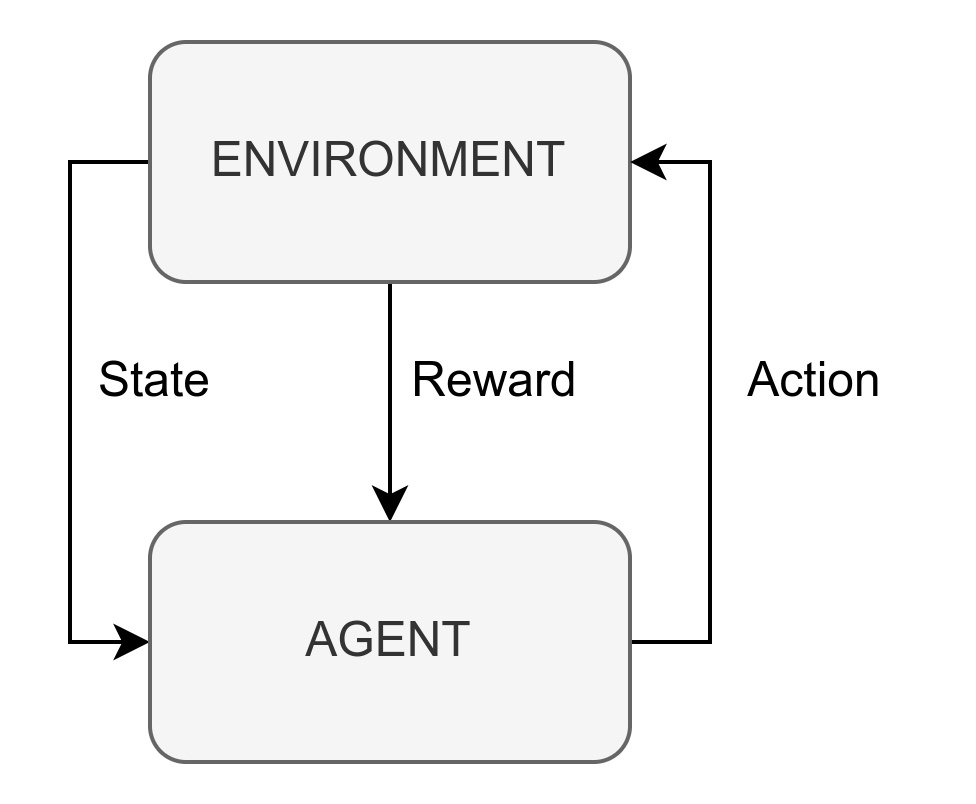
\includegraphics [scale = 0.2]{Images/RL_graph.png}
    \caption{Graph representing reinforcement learning}
    \label{figRL}
\end{figure}
%It can be devided into two strategies for solving said problems. The first strategy involves searching the space or state-action pairs for in order to find which works better in the environment. The second technique is estimating the utillity of a particular action. 
The first concept crucial for reinforcement learning is the \textit{reward function} which is objective feedback from the environment. 
It is usually scalar values that are associated with state-action pairs. 
High rewards are usually associated with state-action pairs which are beneficial for the agent to be situated in whereas negative rewards would then be disadvantageous or \textit{hazardous} states for the agent to be in. 
Essentially what is good and bad for the agent in the environment. The sole objective of the agent is then to maximize this reward \cite{sutton1999reinforcement}.

Naturally, we have to define \textit{state} and \textit{action}, which compared to the rest of the concepts have a very general definition. 
That being the latter is a decision of some sort and the former is all the factors that must be considered when taking an action. 

\subsubsection{Temporal difference learning}

A central class of methods in reinforcement learning is \textit{temporal difference learning} (TD). 
It refers to a class of methods in which learning is based on the difference between temporally successive predictions. 
It aims to adjust the learner's current expectation for the present input pattern so that it more accuratley aligns with the subsequent prediction at the following time step. 
Unlike Monte Carlo and other methods, in TD learning, updates are being performed using the estimated value function every step \cite{tesauro1995temporal}.  
TD methods learn a value function based on a state-action pair, which estimates the expected long-term reward if said action is taken in said state. 

In TD learning includes several submethods or rather algorithms such as SARSA ,Q-learning, TD-Lambda, and others \cite{eiben2007reinforcement}.\\

\subsubsection{Q-learning}
Q-learning is an algorithm in which the environment is modeled as a controlled Markov Decision Process managed by the agent \cite{watkins1992q}. 
The agent chooses an action and accordingly gets rewarded for it. 
It estimates the value of taking an action in a particular state based on immediate rewards and the state-action pair's current \textit{Q value}. 
Q-learning uses Markov chains to calculate the maximum reward that can be accumulated by the next state-action and updates accordingly, as shown in the equation below.

\begin{equation} \label{eqQ}
    { Q(s,a) := Q(s,a) + \eta [r + \gamma \max_{a'} Q(s',a') - Q(s,a)]}
\end{equation}

Equation \ref{eqQ} is the \textit{update} equation which is responsible for mapping estimated long-term rewards to the different state-action pairs. 
Here $Q(s,a)$ is the current state-action of the agent, $r$ is the immediate reward, $\eta$ is the learning rate and $Q(s',a')$ is the next state-action. 
Note that, in Q-Learning, this next action is chosen by greedily selecting the one maximizing future total reward.
An important variable here is $\gamma$ which represents the discount factor. This is used to limit the Markov chain to a limited finite number so they don't end up infinite. This controls how many steps into the future the agent will try to estimate. 


\subsection{Evolutionary computing}
%rewrite
Evolutionary computing comprises computational models based on the concept of evolution and natural selection. 
It includes many different models but the most biologically accurate is Genetic Algorithms \cite{drugan2019reinforcement}. 
Similarly to how organisms evolve by natural selection and sexual reproduction, programs can also simulate these processes and behave in a similar fashion to organisms in order to solve a specific problem. 
Natural selection is the process that determines which individuals get to survive by some test of fitness. After the best fit are selected the creation or reproduction of the next generation starts. 
Reproduction is then the method in which the mixing of genes in the remaining population happens and gets passed to offspring \cite{holland1992genetic}.

\begin{figure}[H]
    \centering
    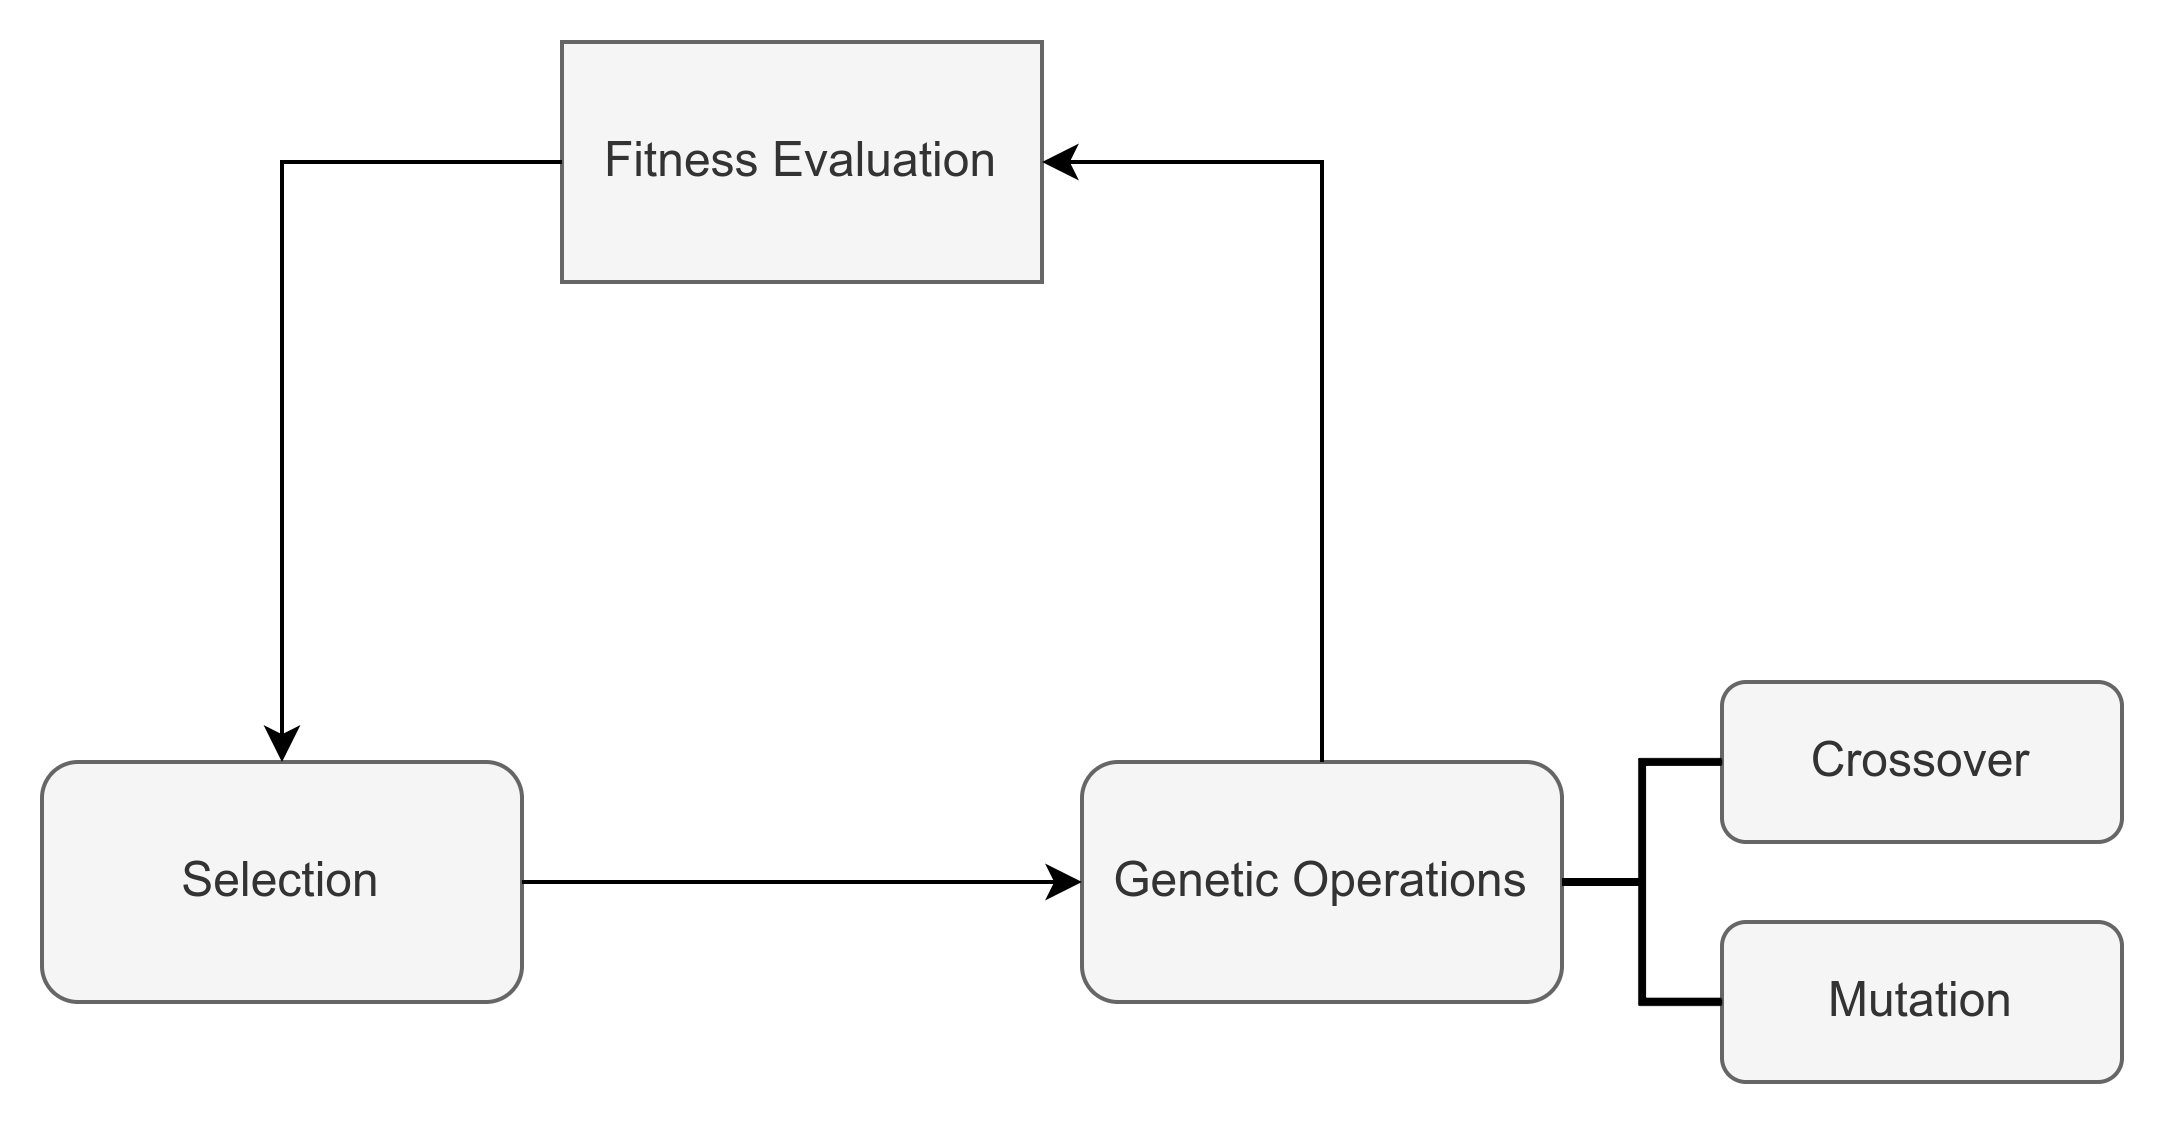
\includegraphics [width=0.5\textwidth]{Images/GA_graph.png}
    \caption{visual representation of genetic algorithms}
    \label{figGA}
\end{figure}

By starting with a randomly created population, we have an initial population with high variation amongst the individuals. 
The \textit{genotype} which is essentially the code of the individual can be represented by a list of instructions. 
These genotypes can be thought of as potential solutions to the problem. 
Due to the variation in the population, some individuals will be better \textit{fit} and thus more likely to be selected to reproduce. 
In the crossover stage, the remaining individuals will mix their genotypes to produce individuals for the next generation. 
These steps will be continuously repeated fore some number of generations \cite{forrest1996genetic}. 

It is important however that we reduce the genetic drift and keep track of the best solutions that have been produced by the previous generation. To do that we employ a method called Elitism. In elitism compared with traditional reproduction the most fitting individuals are copied to the next generation without any alteration. In that way the best solution of each generation is always preserved and adds selective pressure and improves convergence speed \cite{du2018elitism}.

\subsection{Enviroment}
\label{sec:Enviroment}
The environment that will be used to compare the two methods is called cart pole. It is based on the inverted pendulum, a classic control problem that received attention in the field of reinforcement learning in the eighties. The inverted pendulum balances on a cart that ca go either left or right on a horizontal line. The objective is to maintain the balance of the pole by moving the cart. However the movment should be such so the poll remainsbalanced\cite{moriarty1996efficient}.

The goal is to balance a pole on a cart that can move left or right. 
The state space is formally described in Equation \ref{eqStateSpace}, a single vector $s \in \mathbb{S}$ has components $(p, v, \alpha, \omega)$, where $p$ consists of a cart position, $v$ cart velocity, $\alpha$ pole angle, $\omega$ and pole angular velocity.

\begin{equation} \label{eqStateSpace}
{\mathbb{S} = \left\{ s \in \mathbb{R}^4 \mid -4.8 \leq p \leq 4.8, 
 -24^\circ \leq \theta \leq 24^\circ \right\}}
\end{equation}

The action space is discrete, with two possible actions: move left or move right. 

The reward is 1 for every time step the pole is mantained balanced.

The goal is to balance the pole for as long as possible, with a limit of 500 actions.

The environment, called \textit{CartPole-v1}, is implemented in Python using the Gymnasium library \cite{towers_gymnasium_2023}. 
